\documentclass[a0paper,portrait]{baposter}



\usepackage{wrapfig}
\usepackage{lmodern}

\usepackage[utf8]{inputenc} %unicode support
\usepackage[T1]{fontenc}
\usepackage{hyperref}
\usepackage{xcolor}
\usepackage{fontawesome}
\usepackage{multicol}

\hyphenpenalty=10000 % avoid word-splitting (hyphenation)
\selectcolormodel{RGB}

\graphicspath{{figures/}} % Directory in which figures are stored


\newcommand{\compresslist}{%
\setlength{\itemsep}{0pt}%
\setlength{\parskip}{1pt}%
\setlength{\parsep}{0pt}%
}

\newenvironment{boenumerate}
  {\begin{enumerate}\renewcommand\labelenumi{\textbf\theenumi.}}
  {\end{enumerate}}



\begin{document}

\definecolor{loriapink}{RGB}{203,93,155}
\definecolor{loriablue}{RGB}{61,173,226}
\definecolor{loriadark}{RGB}{88,138,181}

\begin{poster}
{
grid=false,
headerborder=open, % Adds a border around the header of content boxes
colspacing=1em, % Column spacing
bgColorOne=white, % Background color for the gradient on the left side of the poster
bgColorTwo=white, % Background color for the gradient on the right side of the poster
borderColor=loriadark, % Border color
headerColorOne=loriadark, % Background color for the header in the content boxes (left side)
headerColorTwo=loriadark, % Background color for the header in the content boxes (right side)
headerFontColor=white, % Text color for the header text in the content boxes
boxColorOne=white, % Background color of the content boxes
textborder=rounded, %rectangle, % Format of the border around content boxes, can be: none, bars, coils, triangles, rectangle, rounded, roundedsmall, roundedright or faded
eyecatcher=false, % Set to false for ignoring the left logo in the title and move the title left
headerheight=0.11\textheight, % Height of the header
headershape=rounded, % Specify the rounded corner in the content box headers, can be: rectangle, small-rounded, roundedright, roundedleft or rounded
headershade=plain,
headerfont=\Large\textsf, % Large, bold and sans serif font in the headers of content boxes
%textfont={\setlength{\parindent}{1.5em}}, % Uncomment for paragraph indentation
linewidth=2pt % Width of the border lines around content boxes
}
{}
%
%----------------------------------------------------------------------------------------
%	TITLE AND AUTHOR NAME
%----------------------------------------------------------------------------------------
%
{\textsf{Controlled Conversational Models through \\ Conversation-Dedicated Ontology}}
{\sf\vspace{0.3em}\\
Barbara Gendron, under the supervision of Mathieu d'Aquin and Gaël Guibon
\vspace{0.1em}\\
\small{Laboratoire Lorrain de Recherche en Informatique et ses Applications (LORIA), Université de Lorraine
\vspace{0.2em}\\
\faEnvelopeO \enspace barbara.gendron@loria.fr | \faDesktop \enspace \url{b-gendron.github.io} | \faGithub \enspace b-gendron | \faLinkedin \enspace barbara.gendron
}}
{
    \makebox[200pt][l]{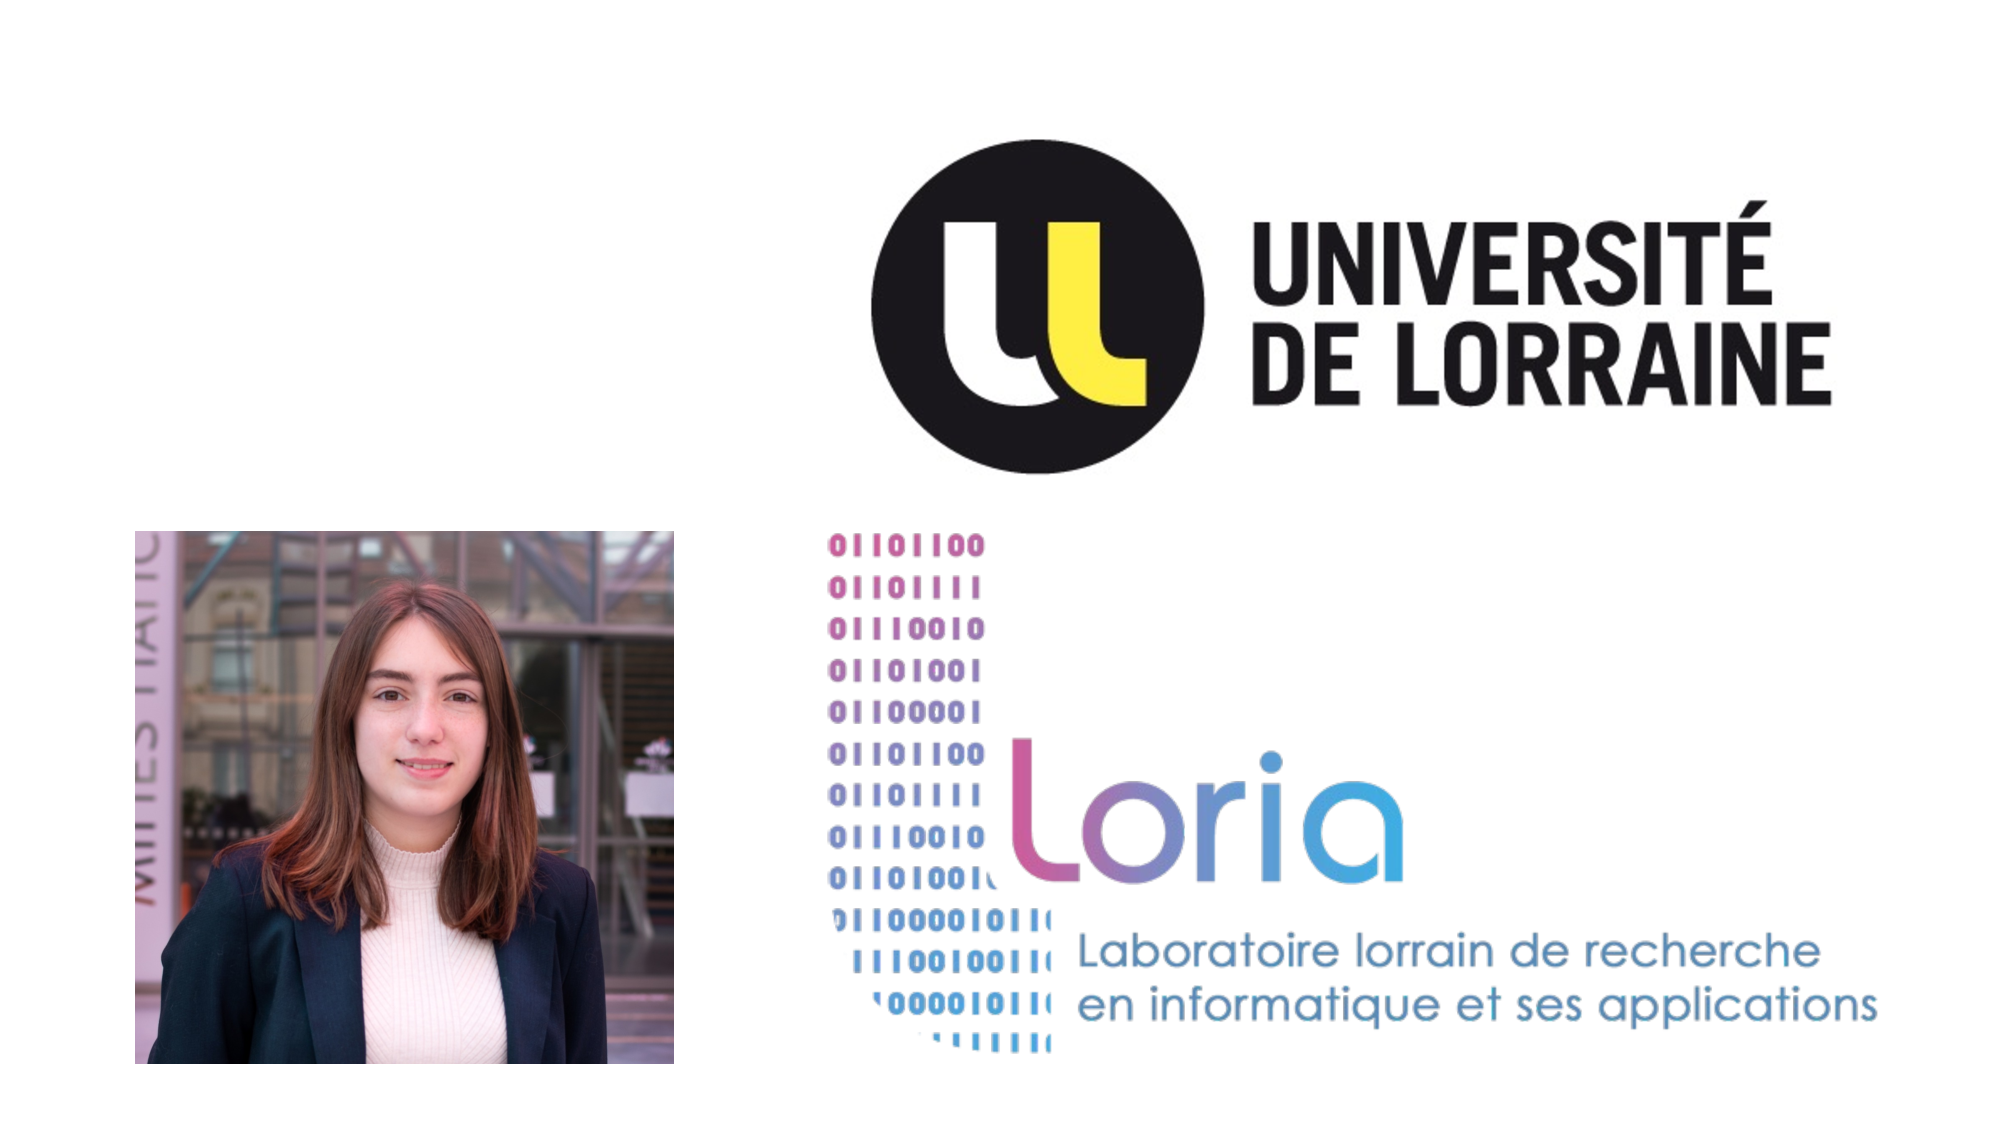
\includegraphics[width=0.28\textwidth]{all-logos-photo.pdf}} 
}%

\headerbox{1. Context}{name=introduction,column=0,row=0, span=3}{

Recent advances in Large Language Models (LLMs) have improved conversational agents' realism and compliance towards human requirements and needs. However, \textbf{controlling conversation flow towards positive outcomes remains crucial}. \\
\\
\noindent This Ph.D. aims to \textcolor{loriapink}{\bf represent conversational knowledge using an ontology to enable language model control}. Ontologies allow to model the knowledge in a domain, defining concepts and characterizing relations between them. While often used for domain-specific knowledge, few have explored using ontologies to guide conversation flow. Convology is a recent example focusing on managing health conversations. We plan to extend Convology's conceptualization capacities to a more general setup, therefore adaptable to general-purpose user/agent conversations.

}

\headerbox{Want to know more?}{name=resources,column=0,below=introduction,span=1}{

\begin{center}
    
\includegraphics[width=0.5\textwidth]{OntoGPT_for_RLA.png}\\
    An example: OntoGPT for Readability Level Assessment (seminar slides)
\end{center}
}

\headerbox{2. Methodology}{name=method,column=0,below=resources,span=1}{

% \paragraph*{PhD approach.} Iterative process by progressive enrichment of the ontology to conceptualize more and more notions related to conversations.\\
\paragraph*{Tools.} Protégé, HermiT and Pellet reasoners, owlready2, rdflib, PyTorch, Huggingface transformers and parameter-efficient fine-tuning libraries, LoRA  and QLoRA adapters.\\
\paragraph*{Ontology.} Progressively incorporate and infer on linguistic features such as part-of-speech tags, affective computing such as emotions or dialog acts.\\
\paragraph*{Experimental Setup.} Toy example design process is a trial and error approach?\\
\paragraph*{Control.} Decisions to use certain outputs rather that other will be directly associated to the ontological dimensions of the current conversation that have driven those choices, which makes the difference with black-box models. In the end, this could help to discourage the generation of harmful content, this bringing controllable ethics to human-machine conversations.\\
\paragraph*{Challenges.} It is not straightforward that the knowledge the ontology brings can be accurately learnt and applied by a language model, whether it be decoder-only or encoder-decoder.

%\vspace{-2pt}
}

\headerbox{3. Motivation \& Objectives}{name=objectives,span=2,column=1,below=introduction}{
The objective of this thesis is to develop \textbf{knowledge-enhanced conversational models} that exploit Large Language Models (LLMs) and Ontologies. This consists in improving state-of-the-art LLMs by providing \textbf{structured knowledge} to open-domain conversational agents.
%%
\begin{wrapfigure}{r}{0.55\textwidth}
    % \vspace{-15pt}
    \begin{center}
        \includegraphics[width=0.5\textwidth]{onto_perspectives.pdf}
        \caption{\centering The benefits of ontology-LLM hybridation systems for conversation modeling}
    \end{center}
\end{wrapfigure}
\noindent\newline\textbf{\large Objectives:}
\begin{itemize}
    \item Build a conversation ontology that accounts for interpersonal relationships concepts and their evolution.
    \item Integrate and assess ontology understanding during fine-tuning.
    \item Bring control on conversational LLM outputs through encapsulated conversation knowledge.
\end{itemize}
\vspace*{10pt}
}


\headerbox{4. OntoGPT: LLM Fine-Tuning Based on Ontology Validation}{name=ontogpt,span=2,column=1,below=objectives}{ % To reduce this block to 1 column width, remove 'span=2'
\vspace*{0.2em}
\textbf{OntoGPT} fine-tunes LLMs using LoRA adapters. It aims at improving generation by learning a classification task guided by the ontology knowledge.
\begin{center}
    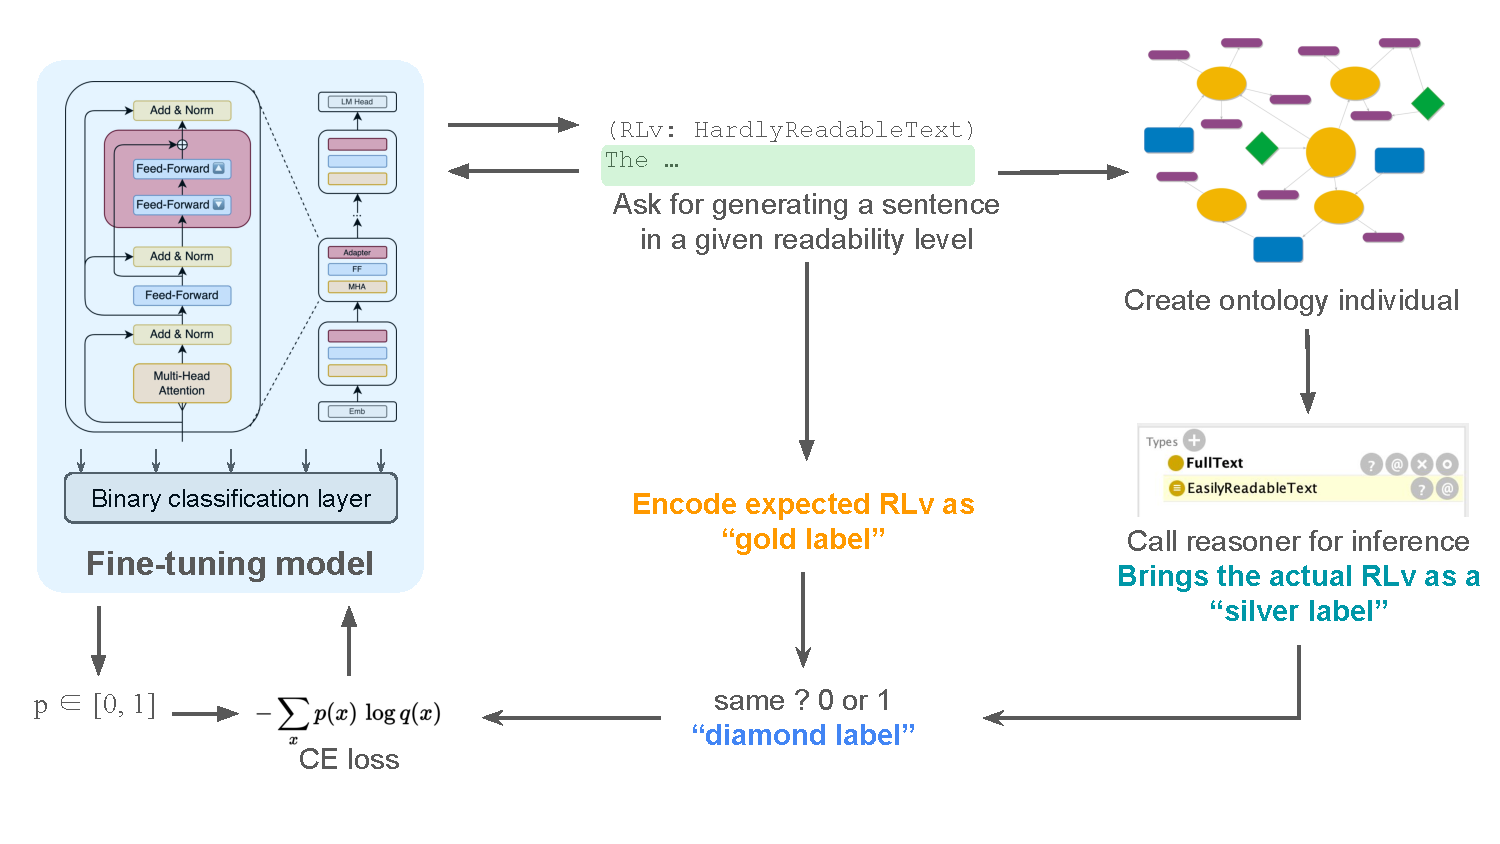
\includegraphics[width=0.95\linewidth]{ft-pipeline.pdf}\\
    \vspace*{0.2em}
    Figure 2: OntoGPT is an end-to-end integration pipeline where the ontology information is assimilated at fine-tuning time. This example focuses on readability level assessment task.
\end{center}
\vspace*{3pt}
}


\headerbox{5. Advances \& Perspectives}{name=rwork,column=0, above=bottom,span=3}{
\begin{tabular}{p{0.3\textwidth} p{0.3\textwidth} p{0.3\textwidth}}
    \begin{minipage}[t]{\linewidth}
        Advances in ontology building:
        \begin{itemize}
            \item Advance 1
            \item Advance 2
        \end{itemize}
    \end{minipage}
    &
    \begin{minipage}[c]{\linewidth}
        \begin{center}
            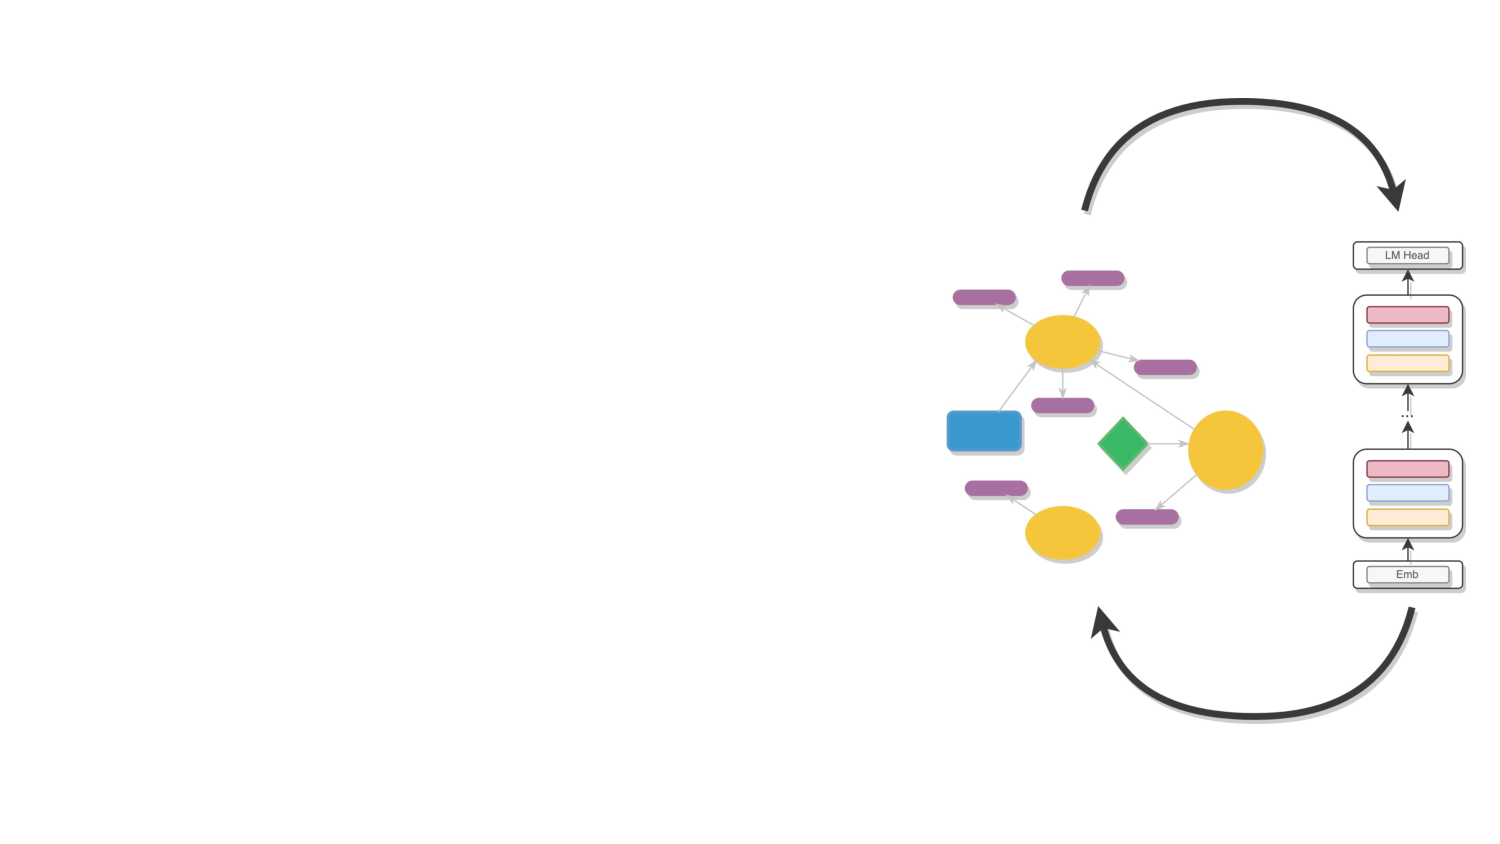
\includegraphics[width=0.55\linewidth]{general-idea.pdf}
        \end{center}
    \end{minipage}
    &
    \begin{minipage}[t]{\linewidth}
        Key findings in LLMs:
        \begin{itemize}
            \item Challenges to setup the fine-tuning procedure
            \item Computational time
        \end{itemize}
    \end{minipage}
\end{tabular}

}


\end{poster}

\end{document}
